\documentclass{report}
\usepackage[utf8]{inputenc}
\usepackage[T1]{fontenc}
\usepackage[brazil]{babel}
\usepackage{graphicx}
\usepackage{amsfonts}
\usepackage{amssymb}
\usepackage{amsmath}
\usepackage{multicol}
\usepackage{ifthen}
\newboolean{firstanswerofthechapter}  
\usepackage{xcolor}
\colorlet{lightcyan}{cyan!40!white}
\usepackage{chngcntr}
\usepackage{stackengine}
\usepackage{tasks}
\usepackage{multirow}
\usepackage{float}
\newlength{\longestlabel}
\settowidth{\longestlabel}{\bfseries viii.}
%\settasks{counter-format={tsk[r].}, label-format={\bfseries}, label-width=\longestlabel,
    %item-indent=0pt, label-offset=2pt, column-sep={10pt}}
		
\setcounter{secnumdepth}{0} \setlength{\topmargin}{0cm}
\setlength{\headsep}{-0.3cm} \setlength{\textwidth}{17.5cm}
\setlength{\textheight}{23cm} \setlength{\oddsidemargin}{-0.8cm}
\setlength{\evensidemargin}{0cm} \setlength{\footskip}{-1.5cm}

		
\usepackage[lastexercise,answerdelayed]{exercise}
%\counterwithin{Exercise}{chapter}
%\counterwithin{Answer}{chapter}
%\renewcounter{Exercise}[chapter]
%\newcommand{\QuestionNB}{\bfseries\arabic{Question}.\ }
%\renewcommand{\ExerciseName}{Exercício}
%\renewcommand{\ExerciseHeader}{\noindent\def\stackalignment{l}% code from https://tex.stackexchange.com/a/195118/101651
    %\stackunder[0pt]{\colorbox{cyan}{\textcolor{white}{\textbf{\LARGE\ExerciseHeaderNB\;\large\ExerciseName}}}}{\textcolor{lightcyan}{\rule{\linewidth}{2pt}}}\medskip}
\renewcommand{\ExerciseName}{Exercícios}
\renewcommand{\ExerciseHeader}{\noindent\def\stackalignment{l}% code from https://tex.stackexchange.com/a/195118/101651
    \stackunder[0pt]{\colorbox{cyan}{\textcolor{white}{\textbf{\large\ExerciseName}}}}{\textcolor{lightcyan}{\rule{\linewidth}{2pt}}}\medskip}
%\renewcommand{\AnswerName}{Exercises}
%\renewcommand{\AnswerHeader}{\ifthenelse{\boolean{firstanswerofthechapter}}%
    %{\bigskip\noindent\textcolor{cyan}{\textbf{CHAPTER \thechapter}}\newline\newline%
        %\noindent\bfseries\emph{\textcolor{cyan}{\AnswerName\ \ExerciseHeaderNB, page %
                %\pageref{\AnswerRef}}}\smallskip}
    %{\noindent\bfseries\emph{\textcolor{cyan}{\AnswerName\ \ExerciseHeaderNB, page \pageref{\AnswerRef}}}\smallskip}}
%\setlength{\QuestionIndent}{16pt}

\begin{document}

\vspace*{-2cm}

\begin{center}
\begin{minipage}[s]{2cm}
\hspace{-1.3cm}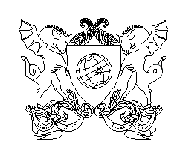
\includegraphics[scale=1.0]{/home/fsbmat/Documentos/GitHub/maf335.github.io/Brasao_UFV/brasaoufv.eps}
\end{minipage}
\begin{minipage}[s]{13cm}
{\begin{center} {\sc \Large Universidade Federal de Vi\c{c}osa}\\
{\sc \large Instituto de Ci\^encias Exatas e Tecnológicas}\\
{\sc \large Campus UFV - Florestal}\\
\end{center}}
\end{minipage}\begin{minipage}[s]{2 cm}
%\includegraphics[width=2 cm]{logoimecc.eps}
\end{minipage}
\end{center}

\vspace{-0.3cm}

%\hline \hline \noindent

%%%%%%%%%%%%%%%%%%%%%%%%%%%%%%%%%%%%%%%%%%%%%%%%%%%%%%%%%%%%%%%%%%%%%%%%%%%

\medskip

\begin{center}

\underline{\underline{{\large{\sc Lista de Álgebra Linear A - Lista 1}}}}

\bigskip

{\large {\bf Prof. Fernando Bastos}}
%\bigskip
%
%%{\sc Data: $19/06/2018$}
\end{center}

\begin{Exercise}

\Question Sejam $A,B\in \mathbb{M}_{m\textrm{x}n}(\mathbb{K}).$ Mostre que:
\begin{tasks}
\task $(A+B)^{t}=A^{t}+B^{t}$
\task $(AB^{t})^{t}=BA^{t}$
\task Se $n=m,$ então $(AB)^{t}=B^{t}A^{t}$
\end{tasks} 

\Question Sejam $A,B\in \mathbb{M}_{n}(\mathbb{K})$ e $\lambda\in \mathbb{R}.$ Mostre que:
\begin{tasks}
\task $det(AB)=detA.detB$
\task $det A=detA^{t}$
\task $det(\lambda A)=\lambda^{n}detA$
\end{tasks} 

\Question Sejam $A,B\in \mathbb{M}_{n}(\mathbb{K})$ matrizes invertíveis. Mostre que:
\begin{tasks}
\task $det(A^{-1})=(detA)^{-1}$
\task $A^{-1}$ é invertível e $(A^{-1})^{-1}=A$
\task $AB$ é invertível e $(AB)^{-1}=B^{-1}A^{-1}$
\end{tasks} 

\end{Exercise}

\end{document}